\documentclass[a4paper]{article}
\usepackage{geometry}
\geometry{margin=1.2in}
\usepackage{hyperref}
\usepackage{subcaption}
\usepackage{graphicx}
\graphicspath{ {./images/} }
\usepackage[table]{xcolor}
  
\begin{document}
  \begin{titlepage}
    \begin{center}
      \vfill
      \textbf{\huge{Skyrmion Trajectory Prediction}} \\
      \vfill
      \hrule
      \vspace{5pt}
      \textbf{\large{University of Manchester}} \\
      \large{Chen Bo Calvin Zhang (10403253)} \\
      \large{Computer Science and Mathematics} \\
      \large{September 26th 2020} \\
      \vspace{5pt}
      \hrule
      \vfill
    \end{center}
  \end{titlepage} 
  
  \tableofcontents
  
  \newpage
  
  \section{Introduction}
  Skyrmions are vortex-like quasiparticles formed in ferromagnets. The aim of the experiments detailed below was to predict the trajectories of the quasiparticles and analyze their behaviour using models that are agnostic of the physics underlying the interaction of skyrmions with the environment.

  The experiments below will investigate the linearity of the relationship between the positions of skyrmions at one time frame and the next, the use of simple linear and polynomial regression model to predict the trajectories further in time, simple recurrent neural network (RNN) models for prediction and the use of a Social Long-Short Term Memory (LSTM) network.

  \section{The Data}
  The data represents a very simple situation in a simple ferromagnet. The skyrmions do not annihilate on the sides of the ferromagnet or against each other. Moreover, no new skyrmions are formed during the simulation.

  The data was provided in two formats:
  \begin{itemize}
    \item as images (one image per frame/time step);
    \item as OVF files, containing $1000\times200$ meshes (one per frame/time step).
  \end{itemize}

  \begin{figure}[h]
    \centering
    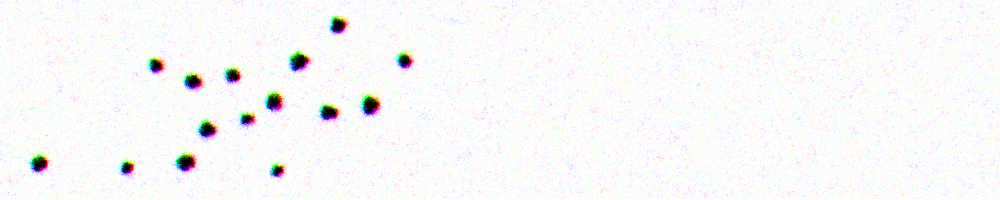
\includegraphics[width=\textwidth]{m000198}
    \caption{Example of image with skyrmions}
    \label{fig:m000198}
  \end{figure}

  In order to extract the coordinates and the trajectories of the skyrmions, both data formats could have been used, but the images (e.g. Figure \ref{fig:m000198}) were chosen as they allowed for less computationally heavy operations on them and for the ease of use. The python library \textit{trackpy} has been used to extract the trajectories from the images.

  First, the skyrmions were detected from each frame (e.g. Figure \ref{fig:m000198_detect}). Consequently, the trajectories were extracted, but since the particles disappearing from the right side of the image would reappear on the left, the problem of different trajectories being detected had to be solved. This issue was solved by considering as the same particle those that disappeared and reappeared with a small displacement on the vertical axis.

  \begin{figure}[h]
    \centering
    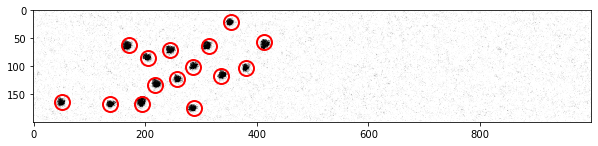
\includegraphics[width=\textwidth]{m000198_detect}
    \caption{Example of image with skyrmions after detecting them with \textit{trackpy}}
    \label{fig:m000198_detect}
  \end{figure}

  Finally, once the number of trajectories matched the number of skyrmions in the initial frame, a \textit{csv} (Table \ref{table:csv}) file was produced. There remained the problem of skyrmions not reappearing for one or two frames (hence not being detected and missing in the \textit{csv} file). This issue was ``solved'' by averaging the positions of the skyrmions before and after the disappearing.

  \begin{table}[h!]
    \centering
    \begin{tabular}{|c c c c|} 
     \hline
     y & x & frame & particle\\ [0.5ex] 
     \hline\hline
     24.42004672 & 61.80999151 & 0 & 0 \\ 
     31.51826059 & 109.0094625 & 0 & 1 \\
     \vdots & \vdots & \vdots & \vdots \\
     180.180794 & 72.36036563 & 0 & 14 \\
     \vdots & \vdots & \vdots & \vdots \\
     93.77902455 & 8679.555818 & 799 & 14 \\
     \hline
    \end{tabular}
    \caption{CSV file containing the data; there are 800 frames and 15 particles, each represented by its x and y coordinates}
    \label{table:csv}
  \end{table}

  \section{Regression}

  \subsection{Experiment 1}
  The aim of the first experiment was to predict the position of the skyrmions in one frame, given the positions in the previous frame.

  First, the data needed to be processed so that we had list representing each frame. The elements of the list were themselves lists, each representing a single frame, in the format $x_0, y_0, x_1, y_1, ...$, where $x_0$ is the x coordinate for the first skyrmion, $y_0$ is the y coordinate for the first skyrmion, $x_1$ is the x coordinate for the second skyrmion, etc.

  The first 80\% of the data was used as training set and the remaining 20\% for testing. Once the training and testing set were obtained, two different models were tried:

  \begin{itemize}
    \item linear regression
    \item polynomial regression of degree 2 with L2 regularization ($\alpha=\frac{1}{2C}=0.5$).
  \end{itemize}

  The performance of the model was then measured using the Root Mean Squared Error ($RMSE$) and $R^2$ metrics.

  \subsubsection{Results}
  The experiment yielded the following results:

  \begin{center}
    \begin{tabular}{ |c|c|c|c|c| } 
     \hline
     Model & $RMSE$ train & $R^2$ train & $RMSE$ test & $R^2$ test \\
     \hline\hline
     Linear & 3.4161 & 0.9854 & 5.9642 & 0.8295 \\ 
     Polynomial & 3.4288 & 0.9893 & 48.3374 & -3.3184 \\ 
     \hline
    \end{tabular}
  \end{center}

  The results are similar on the training set, but it is clear that the polynomial model overfitted the training data, hence performing poorly on the test set. The linear model has greater error and lower $R^2$ in the test set compared to the training set, but this is to be expected. From the results of this experiment we can conclude that there is a close-to-linear relationship between one frame and the next and that the linear model manages to capture a significant amount of the variance of the data.

  Figures \ref{fig:regression1_linear} and \ref{fig:regression1_poly} clearly show that the linear model performs better.
  
  \begin{figure}
    \centering
    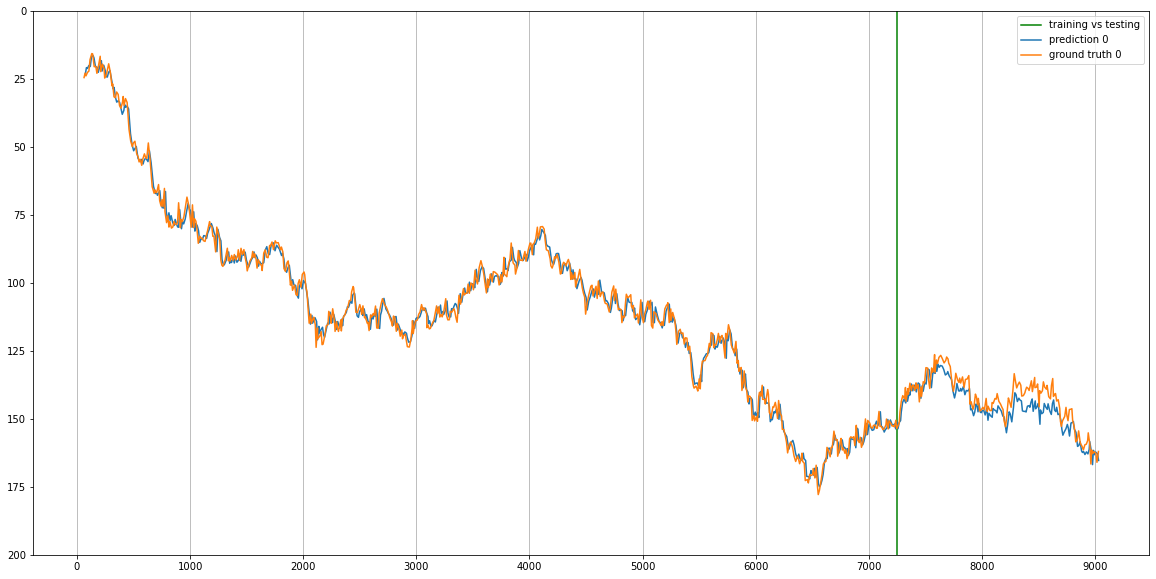
\includegraphics[width=\textwidth]{regression1_linear}
    \caption{Trajectory of the first skyrmion with a linear model}
    \label{fig:regression1_linear}
  \end{figure}

  \begin{figure}
    \centering
    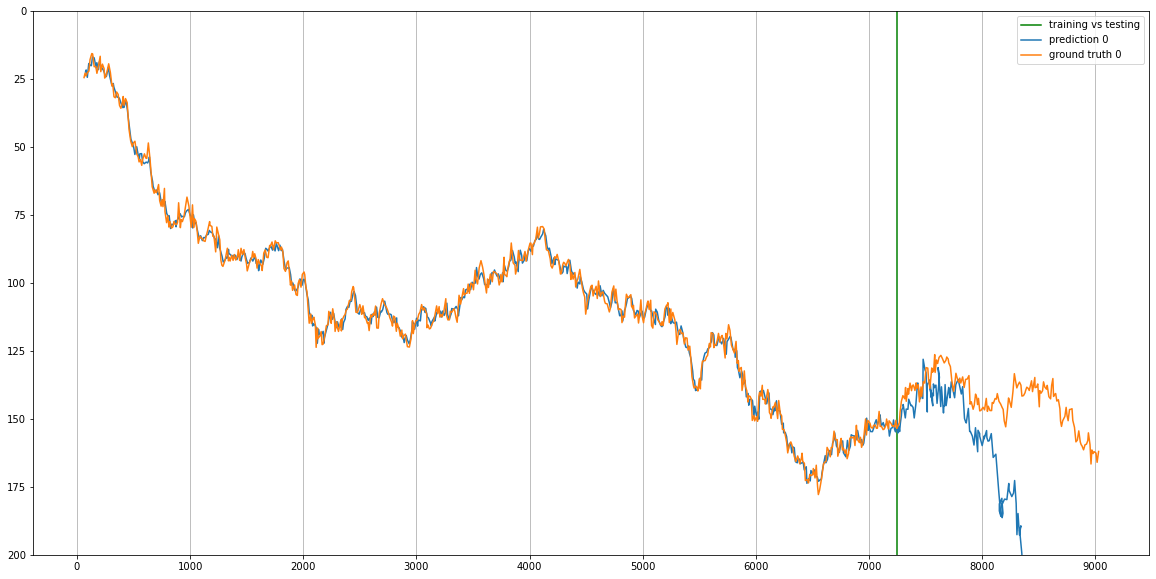
\includegraphics[width=\textwidth]{regression1_poly}
    \caption{Trajectory of the first skyrmion with a polynomial model}
    \label{fig:regression1_poly}
  \end{figure}

  \subsection{Experiment 2}
  The second experiment builds on top of the first one and aims to give better understanding of the linear relationship between one frame and the following ones. In particular, the aim was to find the maximum number $k$ of frames for which the linear relationship lasted.

  The data was structured similarly to experiment 1: the input remained one frame, but the target was now the next $k$ frames. The experiment fitted a linear model for values of $k$ ranging from 1 to 9 computing $RMSE$ and $R^2$ for every value of $k$.

  \subsubsection{Results}
  The table below summarizes the results of the experiment.

  \begin{center}
    \begin{tabular}{ |c|c|c|c|c| } 
     \hline
     k & $RMSE$ train & $R^2$ train & $RMSE$ test & $R^2$ test \\
     \hline\hline
     1 & 3.4161 & 0.9854 & 5.9642 & 0.8295 \\
     2 & 3.6999 & 0.9825 & 7.1709 & 0.7539 \\
     3 & 3.9455 & 0.9799 & 8.5088 & 0.6540 \\
     4 & 4.1535 & 0.9775 & 9.6065 & 0.5617 \\
     5 & 4.3308 & 0.9755 & 10.6797 & 0.4597 \\
     6 & 4.4837 & 0.9737 & 11.6211 & 0.3567 \\
     7 & 4.6172 & 0.9720 & 12.4918 & 0.2588 \\
     8 & 4.7330 & 0.9706 & 13.3560 & 0.1611 \\
     9 & 4.8330 & 0.9692 & 14.1812 & 0.0802 \\
     \hline
    \end{tabular}
  \end{center}

  The table shows that the error is relatively small and we still have a substantial amount of the variance explained for $k \leq 4$, but for greater values, a linear function is not a good approximation any longer.

  \subsection{Experiment 3}
  In this experiment, instead of directly predicting the next $k$ frames, the same linear model from experiment 1 will be used to make successive predictions. Here, the aim is to analyze the maximum number of prediction that can be made before the error propagates too much.

  The nature of the experiment meant that the data also had to have a different format, in particular the data was stored in a DataFrame, where each successive column contained the frames shifted by one time frame.

  \subsubsection{Results}
  In the table below, the value of $k$ represents the number of subsequent predictions made and hence it is expected that the error will propagate and increase quickly.

  \begin{center}
    \begin{tabular}{ |c|c|c| } 
     \hline
     k & $RMSE$ & $R^2$ \\
     \hline\hline
     1 & 5.0975 & 0.9709 \\
     2 & 6.0686 & 0.9579 \\
     3 & 6.8589 & 0.9461 \\
     4 & 7.5293 & 0.9354 \\
     5 & 8.1092 & 0.9256 \\
     6 & 8.6270 & 0.9165 \\
     7 & 9.0881 & 0.9081 \\
     8 & 9.5127 & 0.9002 \\
     9 & 9.9042 & 0.8928 \\
     10 & 10.2683 & 0.8854 \\
     11 & 10.6031 & 0.8787 \\
     12 & 10.9125 & 0.8723 \\
     13 & 11.1982 & 0.86612 \\
     14 & 11.4667 & 0.86019 \\
     15 & 11.7112 & 0.8544 \\
     \hline
    \end{tabular}
  \end{center}

  As the expected, the error increases quickly and for the same number of frames in the future we have a much greater error, but also more variance explained. This is most likely due to the fact that in this case we are making successive prediction from one frame to the next and the linearity holds, whist in experiment 2, we were trying to predict a much higher number of variables, hence probably requiring a more complex function.

  \subsection{Experiment 4}
  This experiment comprised of four sub-experiments:

  \begin{itemize}
    \item A set of randomly chose skyrmions is used for training and the other half is used for testing
    \item The skyrmions in the upper half are used for training and the ones in the lower half are used for testing (and vice versa)
    \item One thirds of the skyrmions is randomly chosen for training and the other two thirds are used for testing
    \item The upper thirds skyrmions are used for training and the middle and lower third skyrmions are used for testing (this experiments has been repeated using the middle thirds and then the lower third for training)
  \end{itemize}

  The set up and of the experiments is identical to the one in experiment 1.

  \subsubsection{Results}

  \paragraph{Random choice of half of the skyrmions for training}
  
  Figure \ref{fig:regression4_random_half} shows the randomly selected skyrmions used for training.

  The table below shows us that the error and $R^2$ score on the training set are similar to the ones in experiment 1. On the test set, we have a similar $R^2$ score, but greater error compared to experiment 1. This can clearly be observed from Figures \ref{fig:regression4_random_half_train_plot} and \ref{fig:regression4_random_half_test_plot} as well.

  \begin{figure}
    \centering
    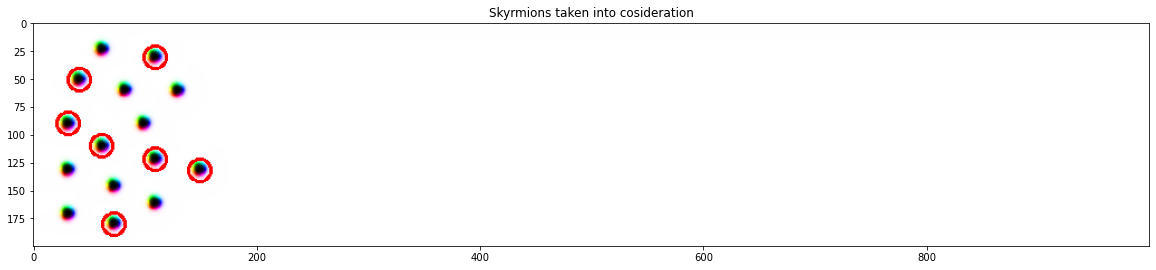
\includegraphics[width=\textwidth]{regression4_random_half}
    \caption{Random choice of half of the skyrmions for training}
    \label{fig:regression4_random_half}
  \end{figure}

  \begin{table}[h!]
    \centering
    \begin{tabular}{|c | c c|} 
     \hline
     Set & $RMSE$ & $R^2$ \\ [0.5ex] 
     \hline\hline
     Train & 3.5384 & 0.9894 \\ 
     Test & 11.1071 & 0.8446 \\
     \hline
    \end{tabular}
  \end{table}

  \begin{figure}
    \centering
    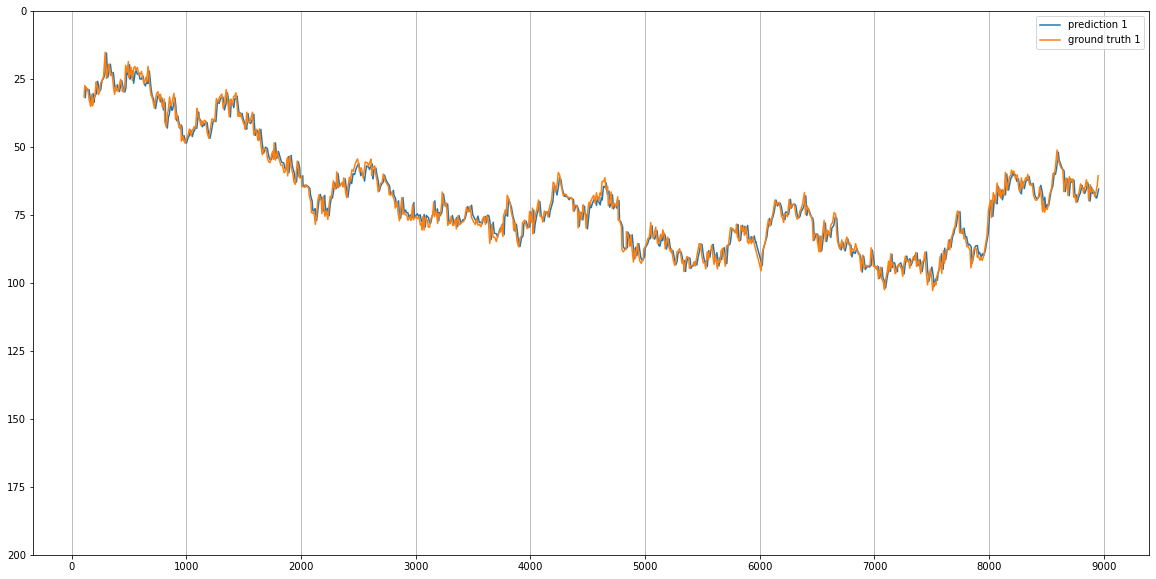
\includegraphics[width=\textwidth]{regression4_random_half_train_plot}
    \caption{Prediction and ground-truth for a skyrmion in the training set}
    \label{fig:regression4_random_half_train_plot}
  \end{figure}

  \begin{figure}
    \centering
    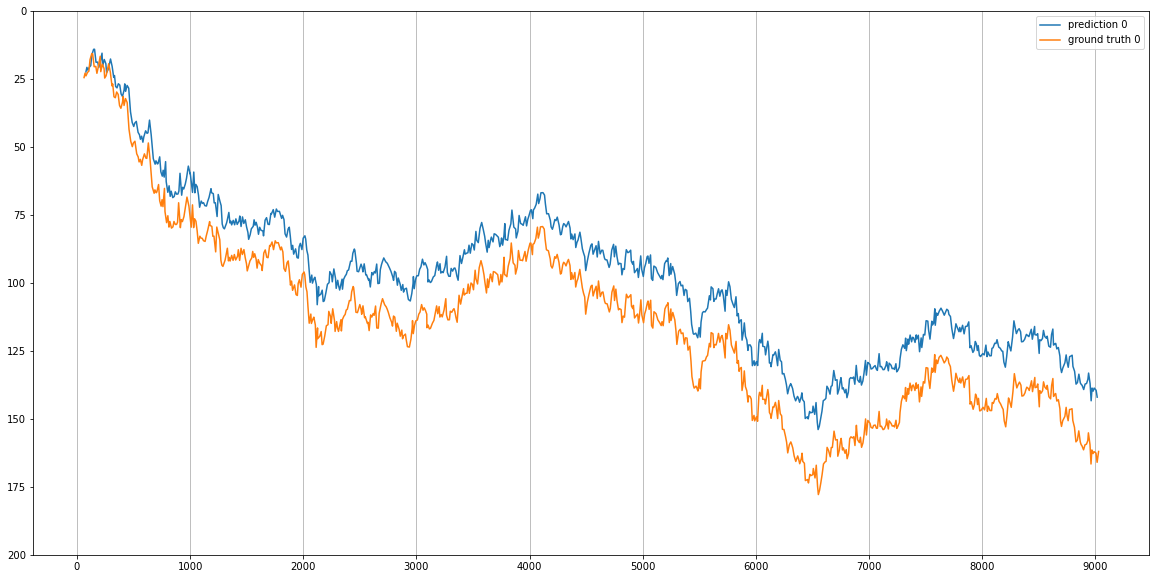
\includegraphics[width=\textwidth]{regression4_random_half_test_plot}
    \caption{Prediction and ground-truth for a skyrmion in the test set}
    \label{fig:regression4_random_half_test_plot}
  \end{figure}

  \paragraph{Top/bottom half for training}

  The table below and Figures \ref{fig:regression4_top_half_train_plot}, \ref{fig:regression4_top_half_test_plot}, \ref{fig:regression4_bottom_half_train_plot} and \ref{fig:regression4_bottom_half_test_plot} show that the errors and the $R^2$ scores are consistent with the previous experiment.

  \begin{table}[h!]
    \centering
    \begin{tabular}{|c|c c|c c|} 
     \hline
     Set used for training & $RMSE$ train & $R^2$ train & $RMSE$ test & $R^2$ test\\ [0.5ex] 
     \hline\hline
     Top & 3.5175 & 0.9889 & 12.2034 & 0.8298 \\ 
     Bottom & 3.5031 & 0.9848 & 11.1262 & 0.8536 \\
     \hline
    \end{tabular}
  \end{table}

  \begin{figure}
    \centering
    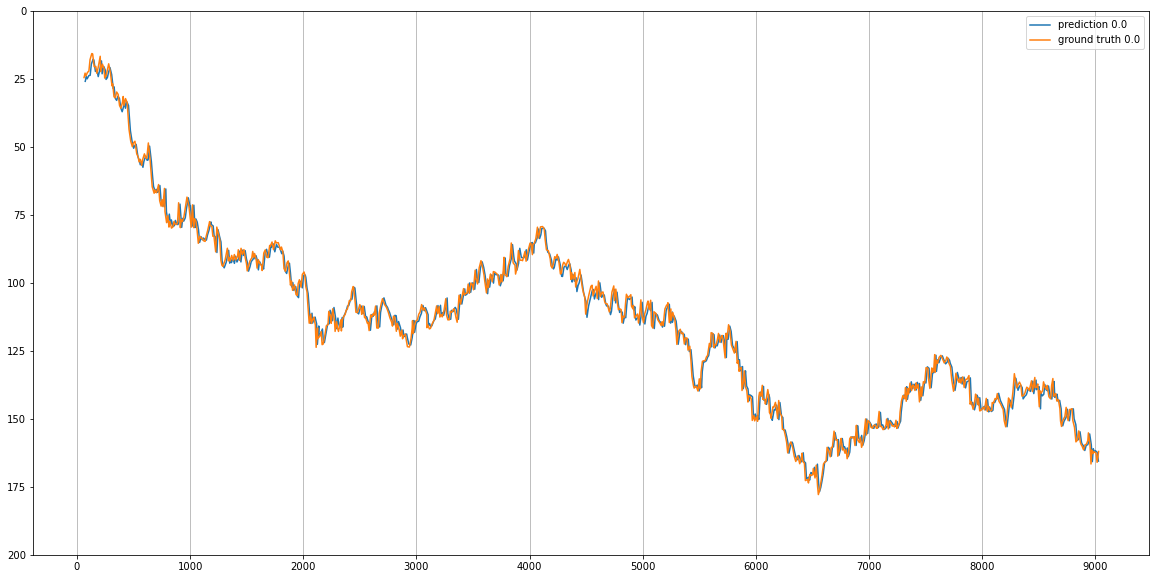
\includegraphics[width=\textwidth]{regression4_top_half_train_plot.png}
    \caption{Prediction and ground-truth for a skyrmion in the train set}
    \label{fig:regression4_top_half_train_plot}
  \end{figure}

  \begin{figure}
    \centering
    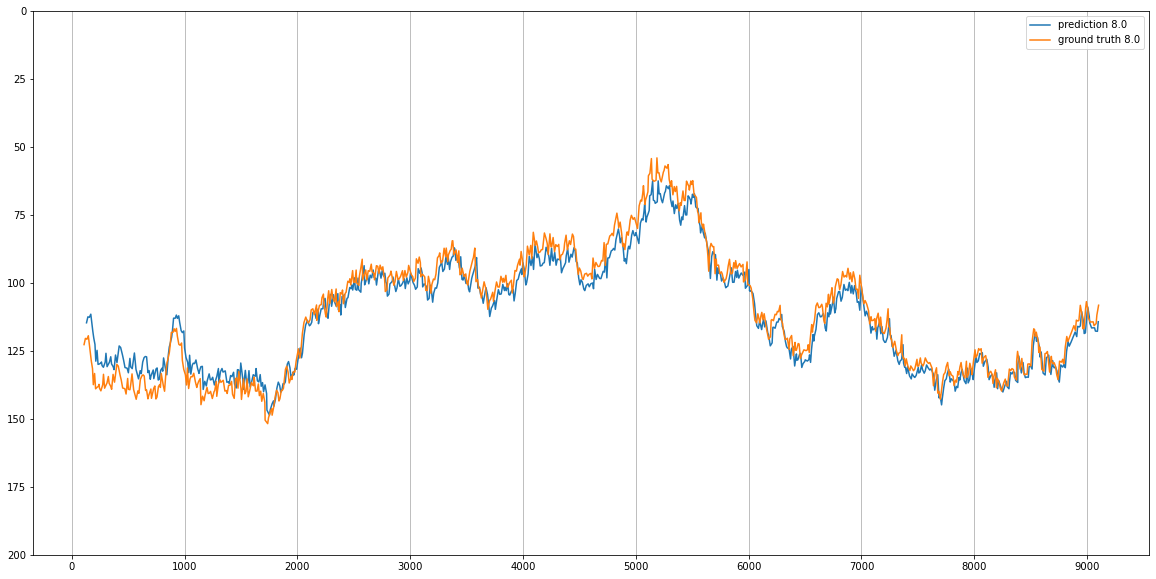
\includegraphics[width=\textwidth]{regression4_top_half_test_plot.png}
    \caption{Prediction and ground-truth for a skyrmion in the test set}
    \label{fig:regression4_top_half_test_plot}
  \end{figure}

  \begin{figure}
    \centering
    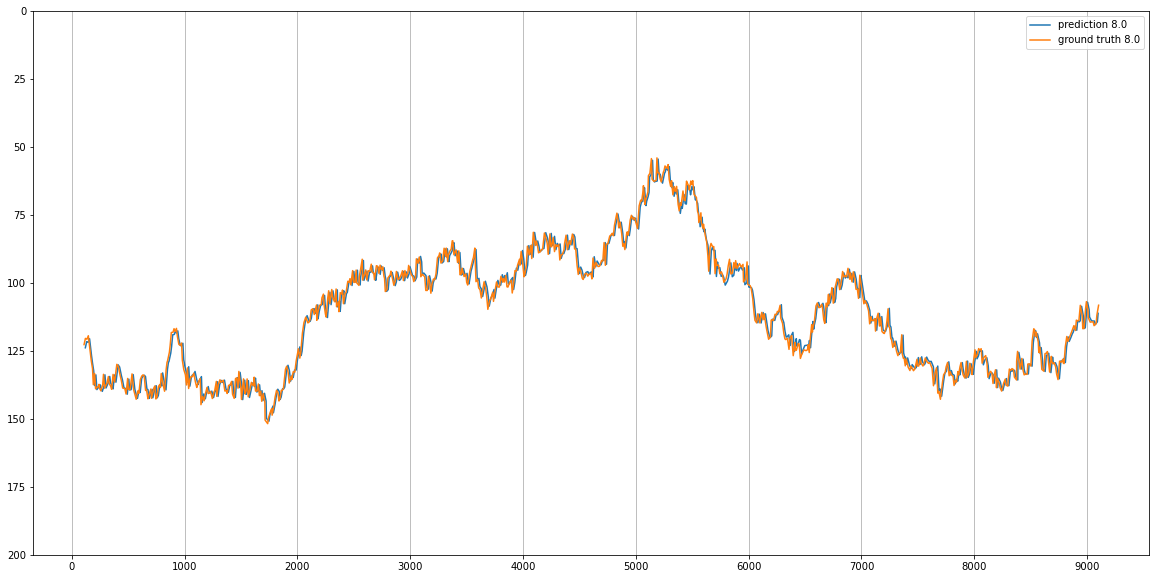
\includegraphics[width=\textwidth]{regression4_bottom_half_train_plot.png}
    \caption{Prediction and ground-truth for a skyrmion in the train set}
    \label{fig:regression4_bottom_half_train_plot}
  \end{figure}

  \begin{figure}
    \centering
    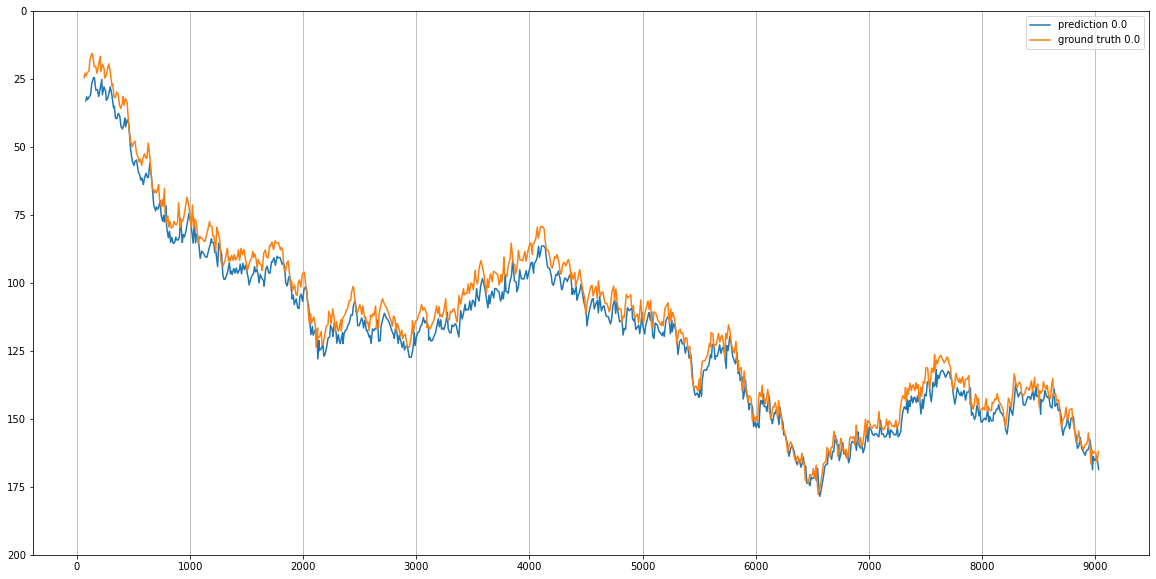
\includegraphics[width=\textwidth]{regression4_bottom_half_test_plot.png}
    \caption{Prediction and ground-truth for a skyrmion in the test set}
    \label{fig:regression4_bottom_half_test_plot}
  \end{figure}

  \paragraph{Random choice of one third of the skyrmins for training}

  Table \ref{table:random_third} below shows that this experiment yielded better results for the test set compared to all the previous experiments. The error on the test set is a bit higher when compared to experiment 1, but the $R^2$ score is much closer to 1, indicating that more of the variance is explained. The improvement on the prediction might be due to the fact that the model is trying to predict fewer coordinates, making the simple linear model perform better.

  \begin{table}[h!]
    \centering
    \begin{tabular}{|c | c c|} 
     \hline
     Set & $RMSE$ & $R^2$ \\ [0.5ex] 
     \hline\hline
     Train & 3.5050 & 0.9806 \\ 
     Test 1 & 7.2381 & 0.9654 \\
     Test 2 & 6.6163 & 0.9533 \\
     \hline
    \end{tabular}
    \caption{Results after training on a random third of the data and testing on the remaining two thirds}
    \label{table:random_third}
  \end{table}

  \paragraph{Top/Middle/Bottom third for training}
  
  The results of this experiment seem to show that a model trained on the centre skyrmions tends to give slightly worse results on the test set. This is interesting because it could give us some insights on how skyrmions interact with each other and the boundaries of the ferromagnet. One hypothesis is that skyrmions which start in the middle might appear to behave more randomly as the lower and upper bound of the ferromagnet are further, hence ``harder'' to reach. Table \ref{table:thirds} below summarizes the results of the experiment.

  \begin{table}[h!]
    \centering
    \begin{tabular}{|c c c c c c|} 
     \hline
     $RMSE$ Top & $R^2$ Top & $RMSE$ Middle & $R^2$ Middle & $RMSE$ Bottom & $R^2$ Bottom \\ [0.5ex] 
     \hline\hline
     \cellcolor{blue!25} 3.5384 & \cellcolor{blue!25} 0.9879 & 8.3660 & 0.9525 & 8.4803 & 0.9032 \\ 
     11.7619 & 0.8922 & \cellcolor{blue!25}3.608 & \cellcolor{blue!25}0.9915 & 11.1467 & 0.9305 \\
     8.6379 & 0.9873 & 8.6264 & 0.9911 & \cellcolor{blue!25}8.4732 & \cellcolor{blue!25}0.9814 \\
     \hline
    \end{tabular}
    \caption{Each row represents a sub-experiment where the highlighted cells contain the values for the training set and the other cells are the values on the test sets ($e.g.$ in the first row, the top third is used for training the the middle and bottom thirds are used for testing).}
    \label{table:thirds}
  \end{table}

  \section{Recurrent Neural Network}
  
  \subsection{Experiment 1}
  This experiment is the same as the first experiment for regression, but a Recurrent Neural Network (RNN) will be used instead. This means that both input and output sequences are 1 time step long. Moreover, the data, unlike in the regression experiments, has been regularized and only two thirds of the date will be used for training.

  The network has the following layers:
  \begin{itemize}
    \item Simple RNN layer with 64 units and a Rectified Linear Unit (ReLU) activation
    \item Dense layer with $n$ ($2 \times $number of skyrmions) units
  \end{itemize}
  and it is optimized using the Adam optimizer and the Mean Squared Error ($MSE$) as loss function. The network was trained for 1000 epochs.

  \subsubsection{Results}
  The model loss decreased sharply in the first few iterations of training on both the training and test set (Figure \ref{fig:rnn1_loss}). The error on the test set continued to decrease until roughly the 200th epoch, after which the improvement was negligible.

  The table below shows us that the predictions are relatively good on the training set, but are extremely poor on the test set. The error on the test set is significantly higher than the error on the training set and the negative $R^2$ score on the test set indicates that no variance of the test set is captured by the model. This can also be clearly seen from Figure \ref{fig:rnn1_plot}, where the prediction for the test set seems to be random.

  \begin{table}[h!]
    \centering
    \begin{tabular}{|c | c c|} 
     \hline
     Set & $RMSE$ & $R^2$ \\ [0.5ex] 
     \hline\hline
     Train & 0.0136 & 0.9746 \\ 
     Test & 0.1077 & -1.3011 \\
     \hline
    \end{tabular}
  \end{table}

  \begin{figure}
    \centering
    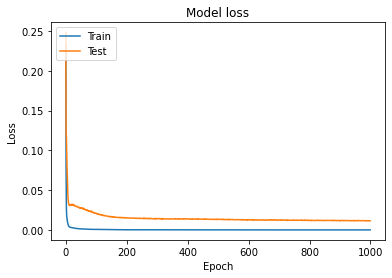
\includegraphics[scale=0.8]{rnn1_loss.png}
    \caption{Training and test set loss}
    \label{fig:rnn1_loss}
  \end{figure}

  \begin{figure}
    \centering
    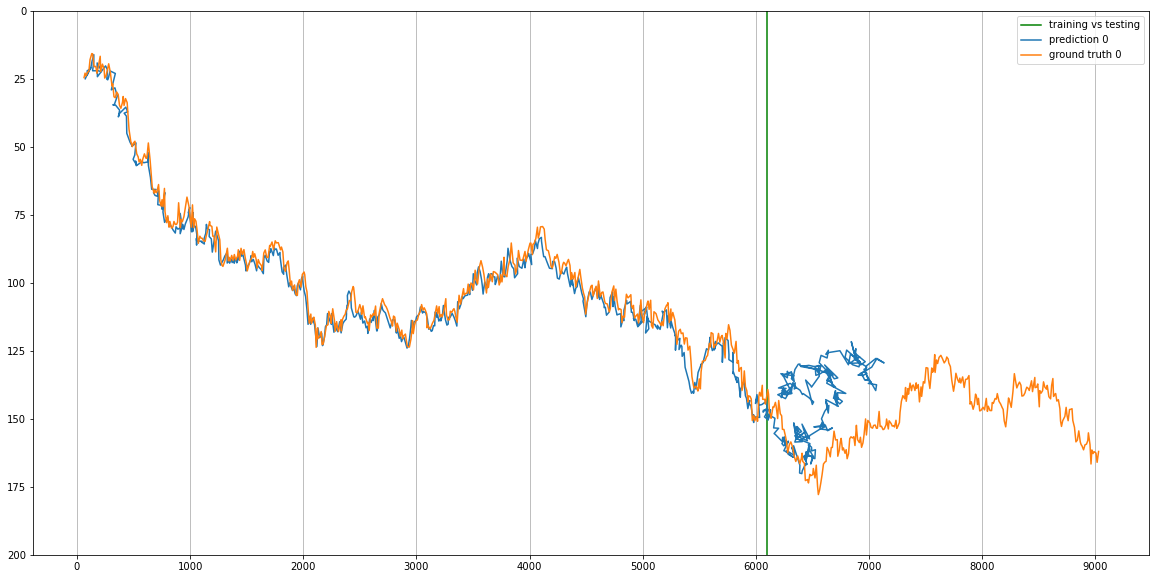
\includegraphics[width=\textwidth]{rnn1_plot.png}
    \caption{Prediction and ground-truth of the first particle}
    \label{fig:rnn1_plot}
  \end{figure}

  \subsection{Experiment 2}
  The complexity of the task of the first RNN experiment might have made it hard for the model to yield good predictions on the test set. In this experiment, only one coordinate will be considered to simplify the task. To further simplify the task, only one particle will be taken into consideration, rather than using all 15 skyrmions.

  The network architecture is as follow:

  \begin{itemize}
    \item Simple RNN layer with 16 units and a Rectified Linear Unit (ReLU) activation
    \item Dense layer with $n$ (in this case it is only 1 as we are predicting one frame in the future for only one coordinate of one skyrmion) units
  \end{itemize}

  The optimizer and the loss function are the same as the previous experiment. The model was trained for 100 epochs.

  \subsubsection{Results}
  As shown in the table below, the model fitted the data very well in both the training and test set. Moreover, the model performs well on other particles as well. Figure \ref{fig:rnn2_loss} shows the training and test loss and \ref{fig:rnn2_plot} and \ref{fig:rnn2_plot_other} show the performance on the training particle and the other particle respectively.

  The results give some questions that can be addressed:

  \begin{enumerate}
    \item How many time steps in the future can we predict?
    \item How does it preform so well even without considering the interaction with other particles? Are particles almost independent in such a simple ferromagnet?
    \item Why is the prediction on another particle also good? Does this mean that the interaction between particles is negligible?
  \end{enumerate}

  \begin{table}[h!]
    \centering
    \begin{tabular}{|c | c c|} 
     \hline
     Set & $RMSE$ & $R^2$ \\ [0.5ex] 
     \hline\hline
     Train & 0.0204 & 0.9843 \\ 
     Test & 0.0196 & 0.9219 \\
     Other particle & 0.0333 & 0.9845 \\
     \hline
    \end{tabular}
  \end{table}

  \begin{figure}
    \centering
    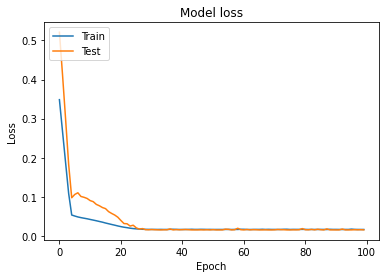
\includegraphics[scale=0.8]{rnn2_loss.png}
    \caption{Training and test loss}
    \label{fig:rnn2_loss}
  \end{figure}
  
  \begin{figure}
    \centering
    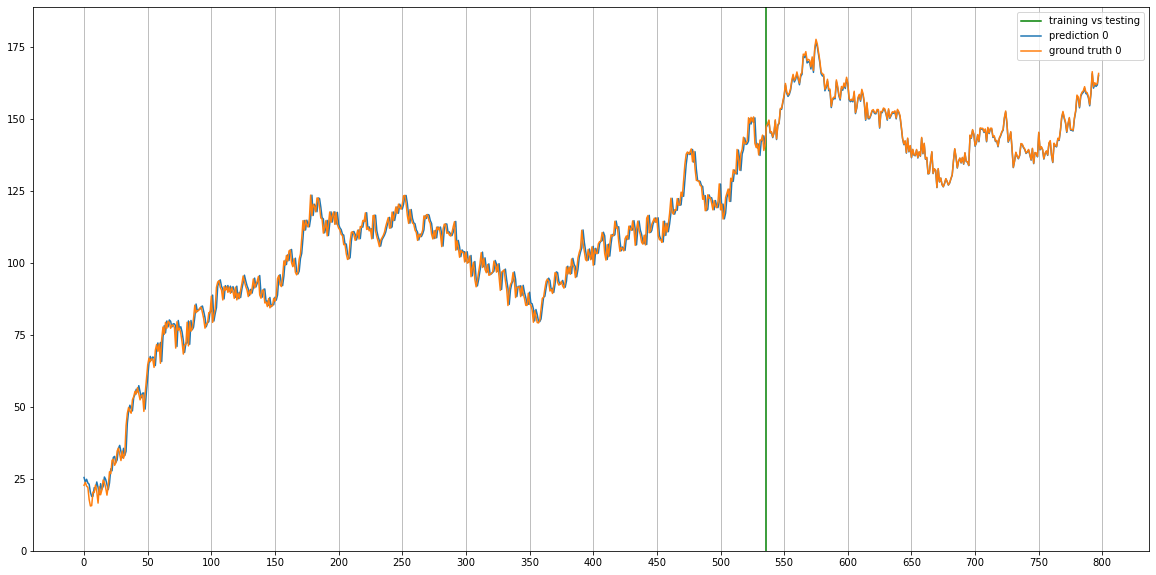
\includegraphics[width=\textwidth]{rnn2_plot.png}
    \caption{Prediction and ground-truth of the first particle}
    \label{fig:rnn2_plot}
  \end{figure}

  \begin{figure}
    \centering
    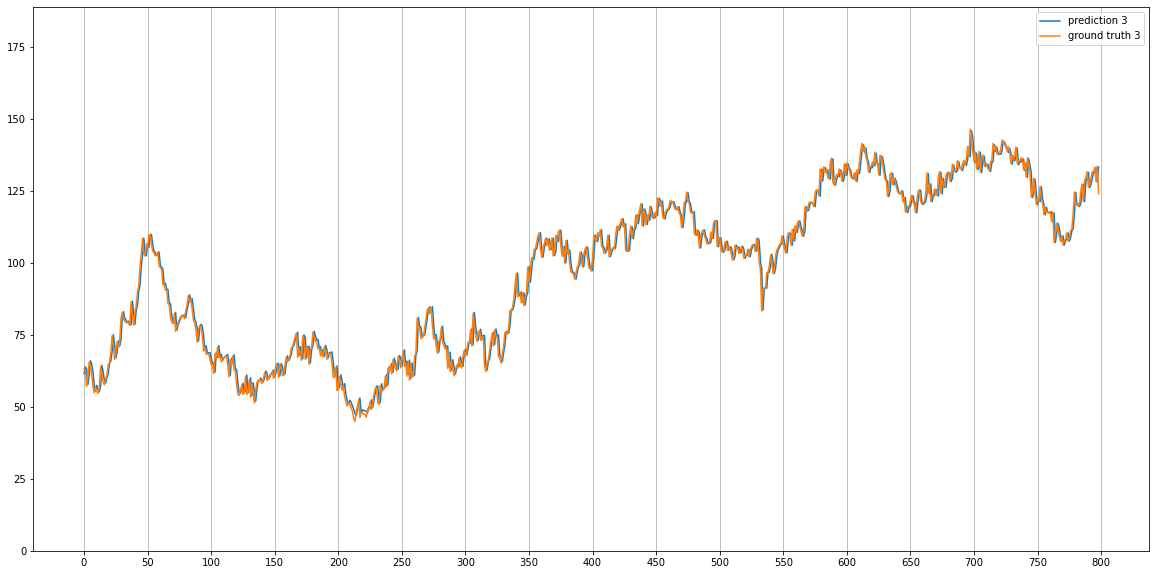
\includegraphics[width=\textwidth]{rnn2_plot_other.png}
    \caption{Prediction and ground-truth of another particle}
    \label{fig:rnn2_plot_other}
  \end{figure}

  \subsection{Experiment 3}
  This experiment has a similar set up to experiment 2, but here the aim is to predict more frames in the future. Two questions need to be answered:

  \begin{enumerate}
    \item How many frames in the past are needed?
    \item How many frames in the future can we predict?
  \end{enumerate}

  The approach consist of starting by setting both the number of past and future frames to 1 and then increasing the number of future frames until the results of the training do not yield good results any longer. Once that happens, the number of frames in the past is increased until the predictions are acceptable again. This process is repeated until a reasonable combination is found.

  The network architecture is as follow:

  \begin{itemize}
    \item Simple RNN layer with 32 units and a Rectified Linear Unit (ReLU) activation
    \item Dense layer with $n$ (i.e. the number of frames in the future as we are working with only one coordinate) units
  \end{itemize}

  The optimizer and the loss function are the same as the previous experiment. The model was trained for 100 epochs.

  \subsubsection{Results}
  A reasonable combination of past and future frames was found when \texttt{n\_past=2} and \texttt{n\_future=7}. The table below summarizes the model performance.

  \begin{table}[h!]
    \centering
    \begin{tabular}{|c | c c|} 
     \hline
     Set & $RMSE$ & $R^2$ \\ [0.5ex] 
     \hline\hline
     Train & 0.0325 & 0.9568 \\ 
     Test & 0.0388 & 0.6998 \\
     \hline
    \end{tabular}
  \end{table}

  The variance captured by the model on the test set is still reasonable, even though it is not performing as well as in the simpler case of predicting only one frame.

  The plots in Figure \ref{fig:rnn3_train} and \ref{fig:rnn3_test} show some predictions on the training and test sets.

  \begin{figure}
    \begin{subfigure}{\linewidth}
      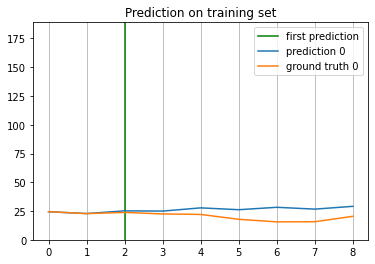
\includegraphics[width=.45\linewidth]{rnn3_train_1.png}\hfill
      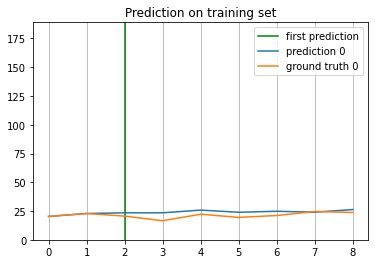
\includegraphics[width=.45\linewidth]{rnn3_train_2.png}\hfill
    \end{subfigure}\par\medskip
    \begin{subfigure}{\linewidth}
      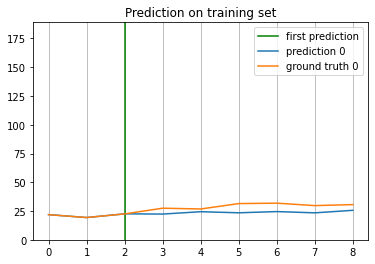
\includegraphics[width=.45\linewidth]{rnn3_train_3.png}\hfill
      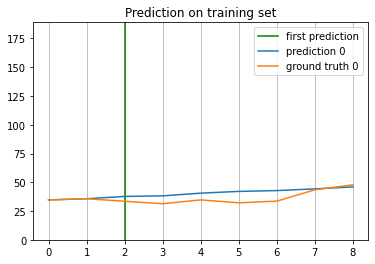
\includegraphics[width=.45\linewidth]{rnn3_train_4.png}\hfill
    \end{subfigure}\par\medskip
    \begin{subfigure}{\linewidth}
      \begin{center}
        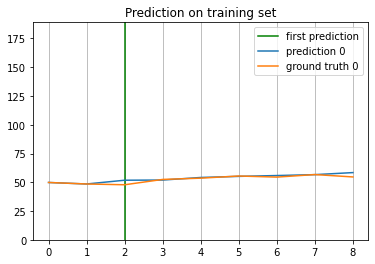
\includegraphics[width=.45\linewidth]{rnn3_train_5.png}
      \end{center}
    \end{subfigure}\par\medskip
    \caption{Predictions of the training set}
    \label{fig:rnn3_train}  
  \end{figure}

  \begin{figure}
    \begin{subfigure}{\linewidth}
      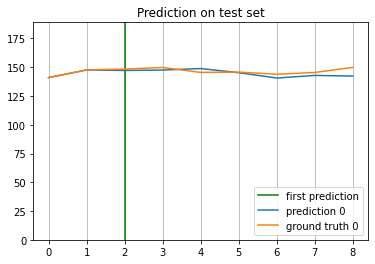
\includegraphics[width=.45\linewidth]{rnn3_test_1.png}\hfill
      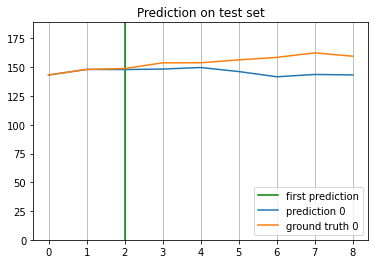
\includegraphics[width=.45\linewidth]{rnn3_test_2.png}\hfill
    \end{subfigure}\par\medskip
    \begin{subfigure}{\linewidth}
      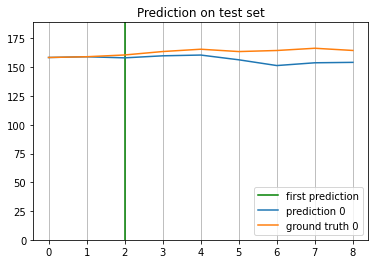
\includegraphics[width=.45\linewidth]{rnn3_test_3.png}\hfill
      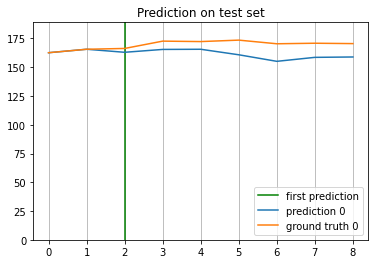
\includegraphics[width=.45\linewidth]{rnn3_test_4.png}\hfill
    \end{subfigure}\par\medskip
    \begin{subfigure}{\linewidth}
      \begin{center}
        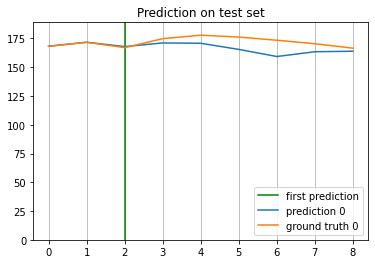
\includegraphics[width=.45\linewidth]{rnn3_test_5.png}
      \end{center}
    \end{subfigure}\par\medskip
    \caption{Predictions of the test set}
    \label{fig:rnn3_test}  
  \end{figure}

  These results show that a Recurrent Neural Network can potentially be used for the prediction of skyrmion trajectories, but that maybe a more complex model (one that manages to explain more variance) is need.

  \subsection{Experiment 4}
  After simplifying the task to only predicting one particle and one coordinate in experiment 2, this experiment aims to test whether it is also possible to use a simple RNN to predict both coordinates for a particle. 

  \begin{itemize}
    \item Simple RNN layer with 16 units and a Rectified Linear Unit (ReLU) activation
    \item Dense layer with $n$ (2 in this case since there are only two dimensions) units
  \end{itemize}

  The optimizer and the loss function are the same as the previous experiment. The model was trained for 250 epochs.

  \subsubsection{Results}
  As expected, the model performs well as the x-axis is close to a linear function, hence easy to learn by a simple model.

  Table \ref{table:rnn4} below shows the results, but plots will not be included as they are similar to the ones for experiment 2.

  \begin{table}[h!]
    \centering
    \begin{tabular}{|c | c c|} 
     \hline
     Set & $RMSE$ & $R^2$ \\ [0.5ex] 
     \hline\hline
     Train & 0.0144 & 0.9921 \\ 
     Test & 0.0140 & 0.9603 \\
     Other particle & 0.02655 & 0.9861 \\
     \hline
    \end{tabular}
    \caption{Results for the model predicting both coordinates of a particle}
    \label{table:rnn4}
  \end{table}

  \section{Social LSTM}
  This experiment is based on the paper \textit{Social LSTM: Human Trajectory Prediction in Crowded Spaces. In CVPR, 2016} by Alahi \textit{et. al.} [\url{http://vision.stanford.edu/pdf/alahi2016cvpr.pdf}].

  The Social LSTM in the paper aims to predict human trajectories given a sequence of past positions by capturing the underlying interactions between people in a crowded space. In our case, we want to capture the subtle interactions between skyrmions, which are different from human ones, but the model should be able to learn them.

  The problem outlined in the paper was that if every person/particle is assigned an LSTM, then the network can learn, but it does not capture the interactions. To solve this problem, a ``Social'' pooling layer is introduced; this layer allows the each network (one for each person/particle) to share hidden states with neighbouring networks.

  \begin{figure}[h]
    \centering
    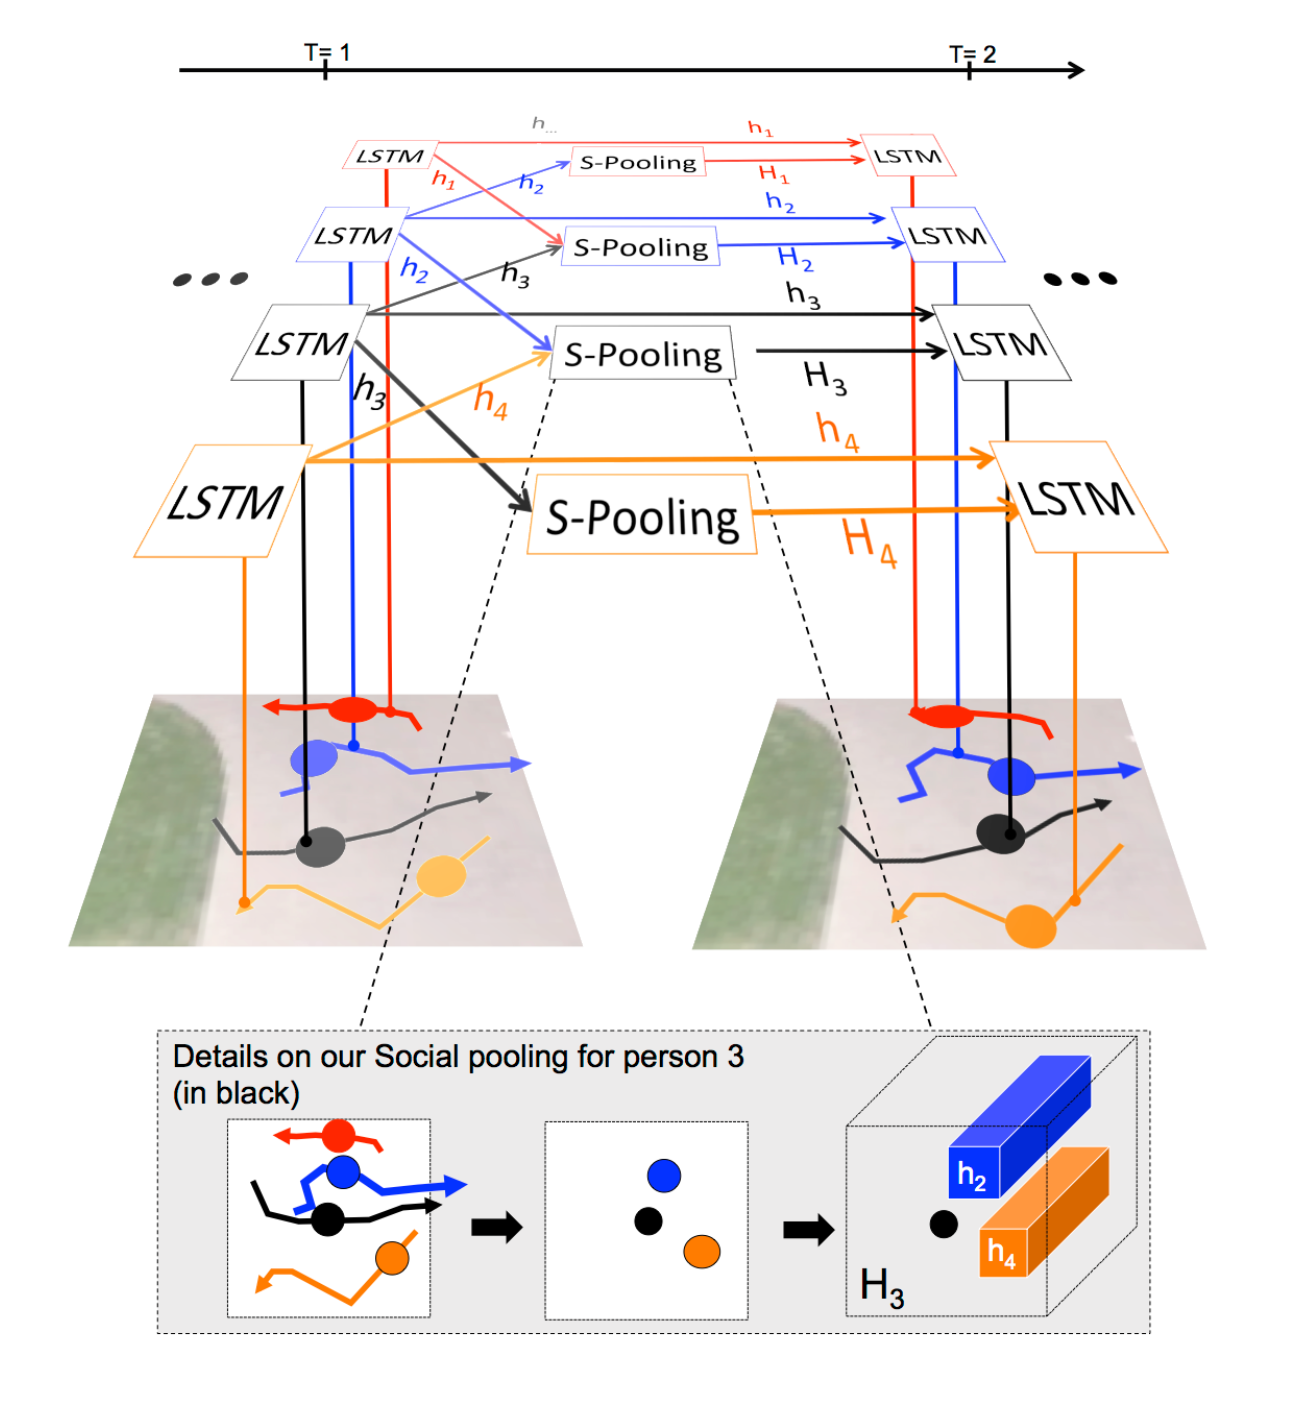
\includegraphics[width=0.45\textwidth]{social_lstm.png}
    \caption{Each person/particle is assigned an LSTM, which are then connected with a Social pooling layer}
    \label{fig:social_lstm}
  \end{figure}

  The data is formatted in the same way as the previous experiments (\textit{i.e.} each frame contains the x and y coordinates for each particle). The model observes positions from frame $i$ to frame $i+T_{obs}$ and predicts frames from $i+T_{obs}+1$ to $i+T_{pred}$.

  The experiment used the implementation found here \url{https://github.com/t2kasa/social_lstm_keras_tf/tree/renew}.

  \subsubsection{Results}
  The experiment did not yield good results as the network architecture needed more hyperparameter tweaking in order to work properly on our case, but the approach seems to promising and should be investigated further.  

\end{document}